	
	\subsection{Лемма Накаямы}

	Пусть $I \subset R$~--- идеал, $M$~--- конечнопорожденный $R$-модуль. 

	Из базового курса алгебры мы знаем такой факт: 

	\begin{theorem}[Гамильтона-Кэли]\label{standard_GK}
		Пусть $A \in \mathrm{M}_{n}(R)$, где $R$~--- коммутативное кольцо. Тогда $\chi_{A}(A) = 0$.
	\end{theorem}

	Докажем теперь некоторое его обобщение. 

	\begin{theorem}[Гамильтона-Кэли]
		Пусть $\varphi \in \End(M)$ такой, что $\Im{\varphi} \subset IM$. Тогда существует многочлен $p(t) = t^n + \alpha_{n - 1}t^{n - 1} + \ldots + \alpha_0$ такой что: 
		\begin{itemize}
			\item $\alpha_i \in I^{n - i}$.
			\item $p(\varphi) = 0$.
		\end{itemize}
	\end{theorem}

	\begin{proof}
		Пусть у модуля $M$ есть $n$ образующих, тогда есть сюръективное отображение $R^n \twoheadrightarrow M$ (а значит и $IR^n \twoheadrightarrow IM$) и вообще есть следующая коммутативная диаграмма: 
		\begin{center}
		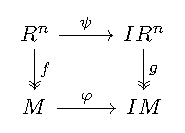
\includegraphics{lectures/3/commutative diagramms/GK.pdf}
 		\end{center}

 		Верхняя стрелка $\psi$ есть из универсального свойства свободного модуля. Так как каждый базисный элемент переходит в элемент с коэффициентами из $I$, $\psi \in M_{n}(I)$. Положим $p = \chi_{\psi}$. Тогда, так как $f$~--- сюръективно, $\forall m \in M \ \exists x\colon f(x) = m$. Тогда:
 		\[
 			p(\varphi)(m) = p(\varphi)(f(x)) = p(\psi)(g(x)) = 0 \implies p(\varphi) = 0.
 		\]
	\end{proof}

	\begin{theorem}[Лемма Накаямы]\label{Nakayama} 
		Пусть $M = IM$. Тогда $\exists a \in M\colon \forall m \in I \  am = m$
	\end{theorem}
	\begin{proof}
		$\id_{M}(M) = IM \implies $, а значит, по теореме Гамильтона-Кэли $\exists p(t) = t^n + \alpha_{n - 1}t^{n - 1} + \ldots + \alpha_0, \ \alpha_i \in I \colon p(\id_{M}) = 0$. Тогда 
		\[
			\id_{M}(1 + \alpha_{n - 1} + \ldots + \alpha_{0}) = 0 \implies \id_{M}(-(\alpha_{n - 1} + \ldots  + \alpha_0)) = 1.
		\]
		Тогда $a = -(\alpha_{n - 1} + \ldots  + \alpha_0)$ подходит. В самом деле, 
		\[
			am = \id_{M}(m) = m \quad \forall m \in M.
		\]
	\end{proof}

	\begin{corollary}
		Если $\varphi \in \End(M)$ и $\varphi$~--- эпиморфизм, то $\varphi$~--- изоморфизм. 
	\end{corollary}

	\begin{proof}
		Определим действие $R[t]$ на $M$ при помощи гомоморфизма $\theta$:
		\[
			\theta\colon R[t] \to \End(M) \quad \theta(t) = \varphi.
		\]

		Так как $\varphi$~--- эпиморфизм, $tR[t]M = M$. 

		Тогда по лемме Накаямы существует $f \in (t) = t R[t]$ такой, что $fm = m \ \forall m \in M$. Запишем $f = tg$ для некоторого $g \in R[t]$ и спроектируем результат в $\End(M)$:
		\[
			t g(t) \cdot m = m \implies \varphi(g(\varphi)(m)) = m \Leftrightarrow \varphi \circ g(\varphi) = \id.
		\]

		Но, по определению, $g(\varphi) = \varphi(g)$, тогда 
		\[
			g(\varphi)(\varphi(m)) = m,
		\]

		$g(\varphi)$~--- обратный к $\varphi$.
	\end{proof}

	\subsection{Радикал Джекобсона}

	Кольцо $R$, рассматриваемое, как модуль над собой, называется \emph{регулярным} $R$-модулем. 

	\begin{definition} 
		Аннулятором $R$-модуля $M$ называется множество $\{ r \in R \ \vert \ rM = 0 \}$.
	\end{definition}

	\begin{lemma} 
		Ненулевой простой $R$-модуль $M$ изоморфен $R/\fm$ для некоторого $\fm \in \Specm{R}$. Таким образом, $\Ann{M}$ является максимальным идеалом кольца $R$. 
	\end{lemma}

	\begin{proof} \ 
	\vspace{30mm}
	\end{proof}




